\chapter{การใช้ชีวิตในประเทศญี่ปุ่น}

สำหรับการฝึกงานร่วมกับมหาวิทยาลัยฮอกไกโดในประเทศญี่ปุ่น ได้ทำการฝึกงานรวมกันเป็นระยะสี่เดือนกับอีกสิบวัน โดยได้เข้ามาทำงานในห้องทดลอง Intelligent Information System ภายใต้การดูแลของอาจารย์ประจำห้องทดลอง \Exami \ และในช่วงเวลาฝึกงานนี้ยังได้รับความช่วยเหลือจากสมาชิกภายในห้องทดลองอีกท่าน Jiang Ye นักศึกษาปริญญาเอก ปี 2 จากประเทศจีน ได้ให้ความช่วยเหลือและการดูแลในเรื่องการดำเนินการเอกสารที่จำเป็นต่าง ๆ เช่น เอกสารการย้ายเข้ามาพำนักในประเทศญี่ปุ่นและการย้ายออกจากประเทศญี่ปุ่น นอกจากนี้ยังได้รับความช่วยเหลือในเรื่องความเป็นอยู่และสิ่งของทั่วไปในการใช้ชีวิตจากทั้งกลุ่มนักศึกษาชาวไทยและชาวต่างชาติซึ่งล้วนศึกษาอยู่ที่มหาวิทยาลัยฮอกไกโด

การใช้ชีวิตในต่างแดน เช่น ประเทศญี่ปุ่นนั้นมีอุปสรรคหลายอย่าง ปัญหาประการหนึ่งที่ประสบบ่อยครั้งที่สุด คือ เรื่องการสื่อสารภาษาญี่ปุ่น อย่างที่ทราบกันดีว่าชาวญี่ปุ่นส่วนใหญ่ไม่สามารถสนทนาภาษาอังกฤษได้ ดังนั้นจึงมีความจำเป็นต้องเรียนรู้ภาษาญี่ปุ่นพื้นฐานเพื่อใช้ในการดำเนินชีวิตประจำวัน รวมถึงสมาชิกภายในห้องทดลองที่ส่วนใหญ่ไม่สามารถสื่อสารด้วยภาษาอังกฤษเช่นกัน สมาชิกภายในห้องทดลองส่วนมากจะสามารถสื่อสารได้เพียงประโยคพื้นฐาน ไม่สามารถสนทนาเป็นบทสนทนาที่ยาวหรือเป็นการเล่าเรื่องได้ แต่อย่างไรก็ดีพวกเขาสามารถอ่านและเขียนภาษาอังกฤษได้ค่อนข้างดี ดังนั้นเมื่อมีปัญหาในการพูดคุยจึงใช้การเขียนหรือพิมพ์ทดแทน อย่างไรก็ดีภายในห้องทดลองก็มีสมาชิกชาวญี่ปุ่นบางคนที่มีความสามารถภาษาอังกฤษในขั้นดีมาก อย่างเช่นนักศึกษาปริญญาโทชาวญี่ปุ่นท่านหนึ่งที่เคยได้ฝึกงานในนิวซีแลนด์และฟิลิปปินส์มาก่อนหน้านี้ทำให้สามารถสื่อสารภาษาอังกฤษได้เป็นอย่างดี

นอกจากตัวผมที่เป็นนักศึกษาฝึกงานจากไทย ภายในห้องทดลองที่ผมฝึกงานก็ยังมีนักศึกษาต่างชาติอีกสองคน คนแรกอย่างที่กล่าวไปในตอนต้น คือ นักศึกษาปริญญาเอกจากประเทศจีน และคนที่สองคือนักศึกษาปริญญาโทจากบราซิล สำหรับชาวจีนนั้นใช้ภาษาญี่ปุ่นเป็นภาษาหลักและสามารถสื่อสารกับคนญี่ปุ่นในห้องทดลองได้อย่างราบรื่น และยังพูดภาษาอังกฤษได้ดีอีกด้วย

\section{ที่อยู่อาศัย}

หอพักที่ใช้อาศัยตลอดโครงการฝึกงานนี้ถูกจัดหาให้โดยทางมหาวิทยาลัยฮอกไกโด หอพักมีชื่อว่า \textit{International House Kita 8 East} เป็นหอชายล้วนจัดให้สำหรับนักศึกษาชาวต่างชาติเท่านั้น โดยภายในห้องจะมีเพียงตู้, เตียง, โต๊ะ, โคมไฟ, ไฟเพดาน, ตู้เย็น, ฮีทเตอร์, และถังขยะ อย่างที่แสดงในภาพ~\ref{Fig:dorm:1} และ~\ref{Fig:dorm:2} สำหรับห้องน้ำ และห้องซักรีดต้องใช้ของส่วนกลางเท่านั้น โดยจะจัดแยกในแต่ละชั้นสำหรับให้ผู้อยู่อาศัยใช้ร่วมกัน

สำหรับห้องครัวและห้องรับประทานอาหารมีจัดเตรียมให้ที่ชั้นแรกของหอพักโดยต้องใช้ร่วมกันทั้งหอพัก เตาแก๊สและอ่างล้างจานถูกติดตั้งไว้เรียบร้อยสามารถใช้งานได้ในทันที สำหรับของใช้ส่วนตัวรวมถึงเครื่องครัวผู้อยู่อาศัยต้องหาซื้อด้วยตนเอง ในกรณีของผมมีความจำเป็นซื้อแค่ชุดจานชามช้อนซ้อมและแก้ว สำหรับอุปกรณ์ทำอาหารได้รับมาจากนักศึกษาชาวจีนที่กำลังจะกลับประเทศจีน ภาพห้องครัวแสดงในภาพ~\ref{Fig:dorm:3} และ~\ref{Fig:dorm:4}

\begin{figure}[!h]
    \centering
    \subfigure[ห้องนอน]{
        \label{Fig:dorm:1}
        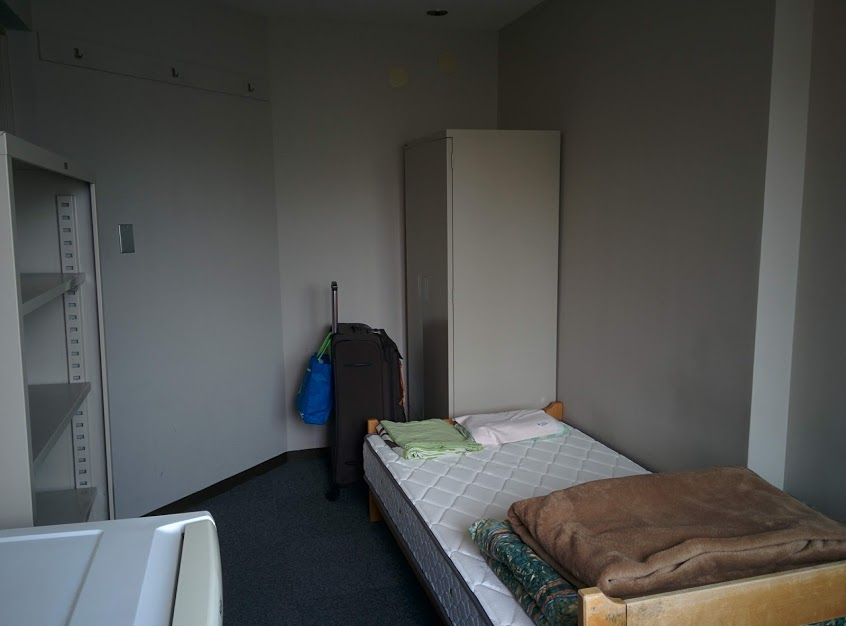
\includegraphics[width=0.45\linewidth]{dorm1}
    }
    \subfigure[ห้องนอน]{
        \label{Fig:dorm:2}
        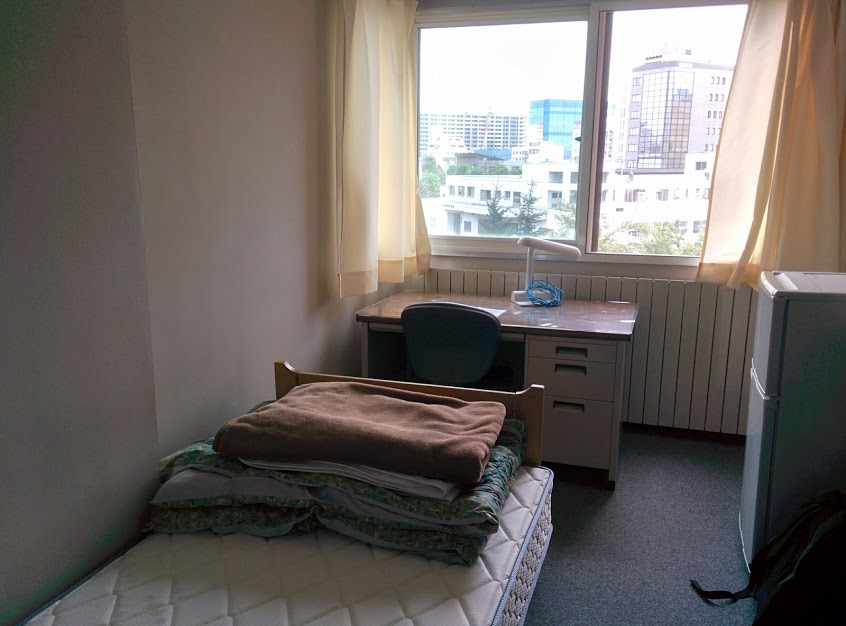
\includegraphics[width=0.45\linewidth]{dorm2}
    }
    \subfigure[ห้องอาหาร]{
        \label{Fig:dorm:3}
        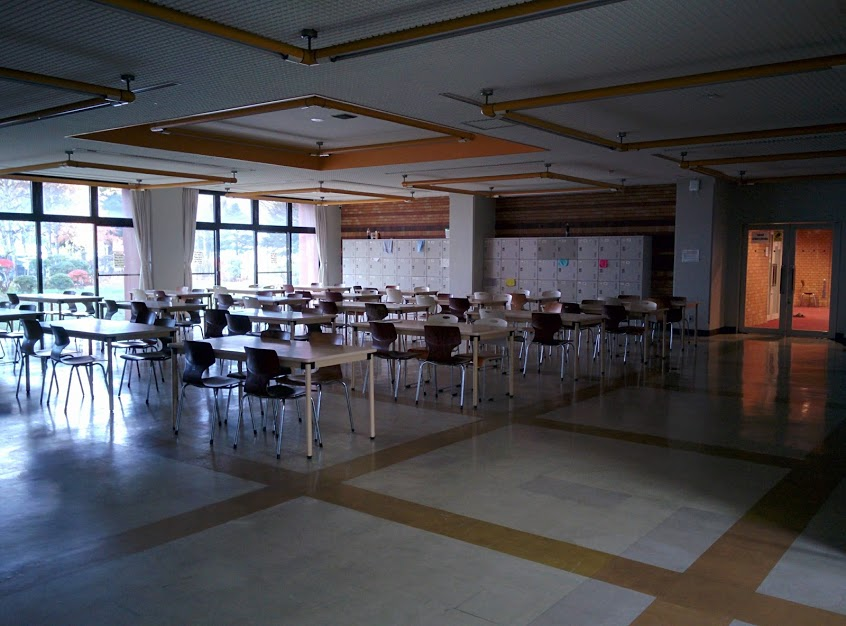
\includegraphics[width=0.45\linewidth]{dorm4}
    }
    \subfigure[ห้องครัว]{
        \label{Fig:dorm:4}
        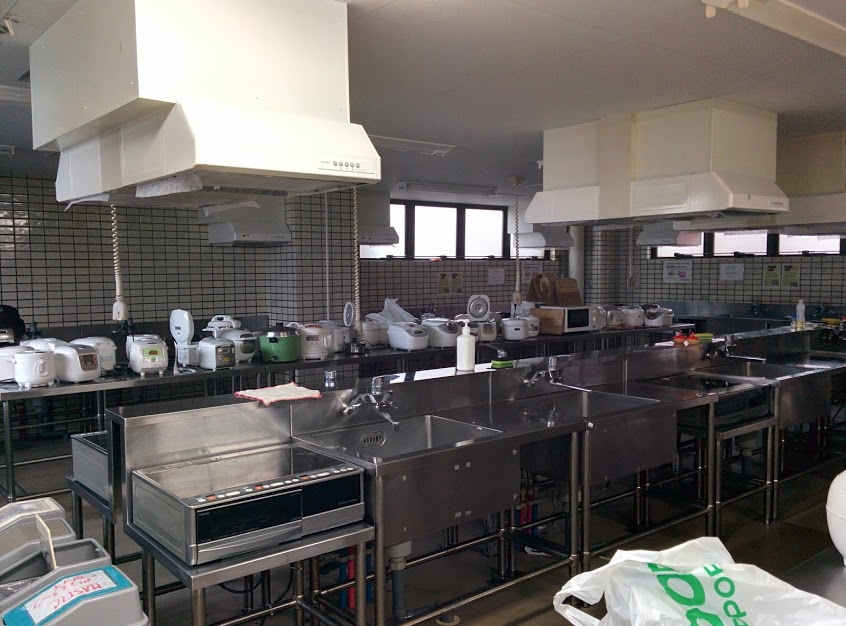
\includegraphics[width=0.45\linewidth]{dorm3}
    }
    \caption{ภาพหอพัก International House Kita 8 East}
    \label{Fig:dorm}
\end{figure}

\chapter{กิจกรรมระหว่างฝึกงาน}

นอกจากการมาทำโปรเจคแล้วนั้น ระหว่างสี่เดือนนี้ผมยังได้ร่วมกิจกรรมด้านวิชาการต่าง ๆ ดังเช่น การประชุมห้องทดลองรายสัปดาห์ และ การร่วมนำเสนอผลงานระหว่างห้องทดลอง เป็นต้น โดยรายละเอียดจะกล่าวต่อจากนี้

\section{Mirai Symposium}

กิจกรรมนี้จัดขึ้นที่เรียวกังหรือรีสอร์ทแบบญี่ปุ่น ซึ่งมีออนเซ็นหรือบ่อน้ำพุร้อนให้ได้แช่อีกด้วย ค่าใช้จ่ายทั้งหมดทางห้องทดลองออกให้ทั้งหมด ภายในงานจะมีกิจกรรมหลักคือการให้นักศึกษาทุกคนของห้องทดลองต่าง ๆ ที่มาร่วมงานนำผลงานตนเองมานำเสนอด้วยโปสเตอร์ในห้องประชุม หมุนเวียนไปเป็นช่วงเวลาคนละ 30 นาที หากสนใจงานของใครก็สามารถเดินไปสอบถามได้ อย่างที่เห็นในภาพ~\ref{Fig:mirai:1} การนำเสนอไม่ได้จำกัดว่างานต้องเป็นผลงานที่เสร็จสิ้นแล้ว อาจเป็นความก้าวหน้าของงานที่พัฒนาอยู่ได้เช่นเดียวกัน สำหรับครั้งนี้มีห้องทดลองร่วมงานสามห้องทดลอง สำหรับนักศึกษาต่างชาติจะมีนักศึกษาท่านอื่นเข้ามาสอบถามเพียงเล็กน้อยเนื่องจากต้องสื่อสารด้วยภาษาอังกฤษและนักศึกษาญี่ปุ่นส่วนใหญ่ไม่สามารถพูดอังกฤษได้ สำหรับงานวิจัยที่ผมพัฒนาก็ได้นำไปนำเสนอในงานนี้ด้วยเช่นเดียวกัน

เมื่อช่วงนำเสนอเสร็จสิ้น ทุกคนจะได้พักผ่อนตามอัธยาศัยโดยส่วนใหญ่จะเลือกไปแช่บ่อน้ำพุร้อนกัน สำหรับบ่อน้ำพุร้อนก็มีทั้งภายนอกและภายในอาคาร จากนั้นเป็นมื้อเย็นซึ่งเป็นอาหารชุดญี่ปุ่น~\ref{Fig:mirai:2}

\begin{figure}[!h]
    \centering
    \subfigure[บรรยากาศระหว่างการนำเสนอผลงานด้วยโปสเตอร์]{
        \label{Fig:mirai:1}
        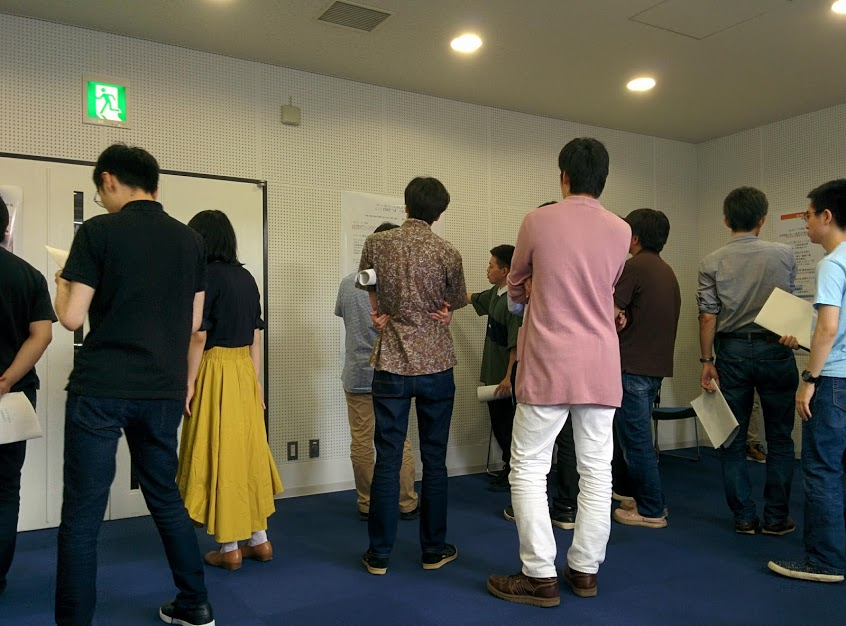
\includegraphics[width=0.8\linewidth]{mirai1}
    }
    \subfigure[ชุดอาหารจัดเลี้ยงมื้อเย็น]{
        \label{Fig:mirai:2}
        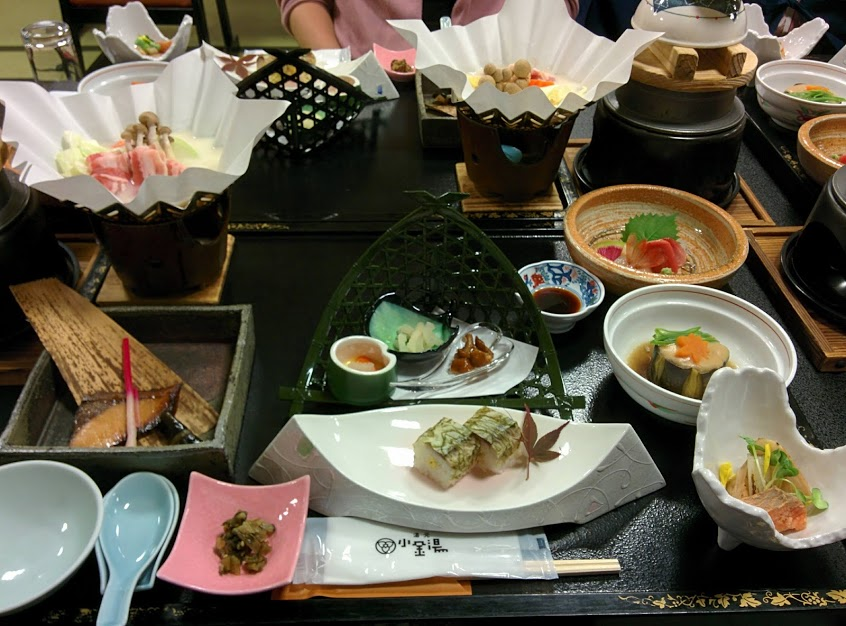
\includegraphics[width=0.45\linewidth]{mirai2}
    }
    \subfigure[ห้องอาหารจัดเลี้ยง]{
        \label{Fig:mirai:3}
        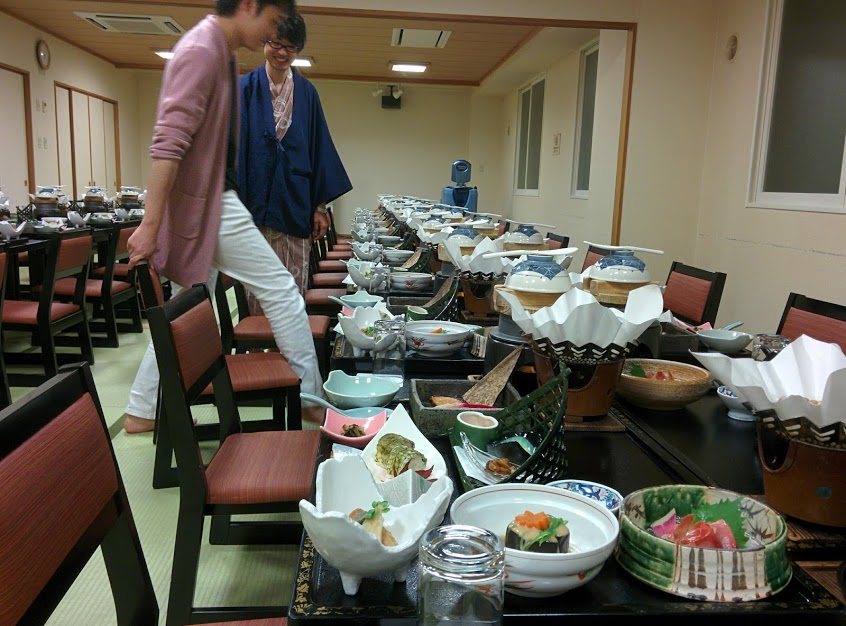
\includegraphics[width=0.45\linewidth]{mirai3}
    }
    \caption{ภาพกิจกรรมในงาน Mirai Symposium}
    \label{Fig:mirai}
\end{figure}

สำหรับวันที่สองก็มีกิจกรรมสร้างสรรค์ เป็นกิจกรรมที่ให้แยกกลุ่มกันและแก้โจทย์ปัญหาโดยให้แก้ภายในเวลาที่กำหนด ตัวอย่างคำถามเช่น \textit{มีเหรียญอยู่ร้อยเหรียญมีทั้งที่หงายหน้าก้อยและหัวอย่างละครึ่ง ต้องการแบ่งกลุ่มเหรียญสองกลุ่มโดยที่แต่ละกลุ่มมีจำนวนหน้าเหรียญและก้อยเท่า ๆ กัน โดยที่ผู้แบ่งมองไม่เห็นเหรียญจะทำได้อย่างไร} เป็นต้น เมื่อเสร็จกิจกรรมสร้างสรรค์ก็ถือเป็นการจบกิจกรรม Mirai Symposium แต่เพียงเท่านี้และเดินทางกลับมหาวิทยาลัย

\section{Lab Meeting}

สำหรับท้องทดลองที่ได้เข้ามาฝึกงานนั้นมีกิจกรรม Lab Meeting ทุกวันพุธ คือ กิจกรรมที่ให้สมาชิกภายในห้องทดลองร่วมกันนำงานวิจัยต่าง ๆ ที่ได้อ่านมานำเสนอต่อสมาชิกท่านอื่น ๆ ภายในห้องทดลอง โดยแต่ละสมาชิกจะถูกกำหนดวันเพื่อให้แต่ละคนที่ถูกกำหนดในวันนั้นนำ Conference Paper หรือ Journal ที่ถูกตีพิมพ์ในงานประชุมวิชาการชื่อดังของโลกมาร่วมกันนำเสนอแบบสรุปพร้อมสไลด์ กิจกรรมนี้ไม่มีคะแนนหรือรางวัลใด ๆ แต่เป็นการแลกเปลี่ยนความรู้ที่เกี่ยวข้องกับงานของตนเองที่ทำอยู่ 

สำหรับผมได้มีโอกาสนำเสนองานวิจัยที่ถูกตีพิมพ์ใน Journal เรื่อง \textit{Text-aware balloon extraction from manga} โดยหลังจากนำเสนอเสร็จสิ้นก็ได้รับคำถามและความคิดเห็นจากสมาชิกและอาจารย์ของห้องทดลองอย่างหลากหลาย ซึ่งถือเป็นโอกาสที่ดีในการเรียนรู้มุมมองและความคิดเห็นที่แปลกใหม่ต่องานของเรา

\section{กิจกรรมอื่น ๆ}

นอกจากกิจกรรมเชิงวิชาการแล้ว ผมยังได้ร่วมในกิจกรรมสังสรรค์อื่น ๆ เช่น งานเลี้ยงตามโอกาสต่าง ๆ โดยผมได้ร่วมงานเลี้ยงต้อนรับตัวผม ซึ่งจัดในช่วงเดือนตุลาคมที่ผ่านมา สาเหตุที่จัดช้าจากเดือนที่เข้าฝึกงานวันแรกไปหลายเดือนเนื่องจากกำหนดการในตอนแรกนั้นคือหนึ่งเดือนหลังจากผมมาอยู่ที่ประเทศญี่ปุ่น แต่ในช่วงกำหนดการเกิดเหตุการณ์แผ่นดินไหวใหญ่บนเกาะฮอกไกโดทำให้ต้องเลื่อนกำหนดการออกไป โดยงานเลี้ยงนี้จัดที่ร้านเนื้อย่างเจงกิสข่าน เป็นเนื้อแกะย่างบนเตาเหล็กลักษณะคล้ายหมูกระทะในประเทศไทยแตกต่างกันเพียงเน้นไปที่เนื้อแกะเป็นหลัก ภาพกิจกรรมแสดงในภาพ~\ref{Fig:welcome-party}

\begin{figure}[!h]
    \centering
    \subfigure[สมาชิกในห้องทดลองระหว่างกินเลี้ยง]{
        \label{Fig:welcome-party:1}
        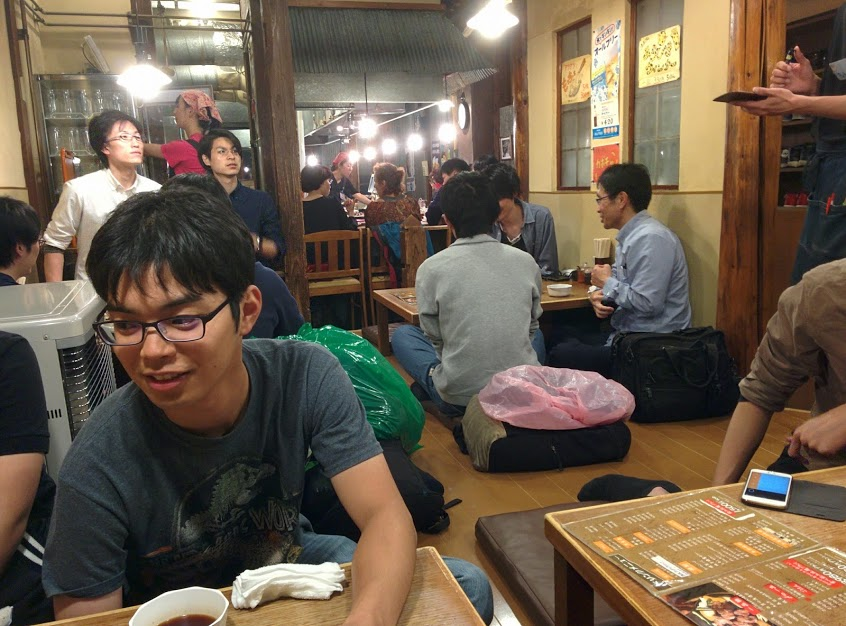
\includegraphics[width=0.8\linewidth]{welcome-party-1}
    }
    \subfigure[โต๊ะอาหารในร้านอาหารเจงกิสข่าน]{
        \label{Fig:welcome-party:2}
        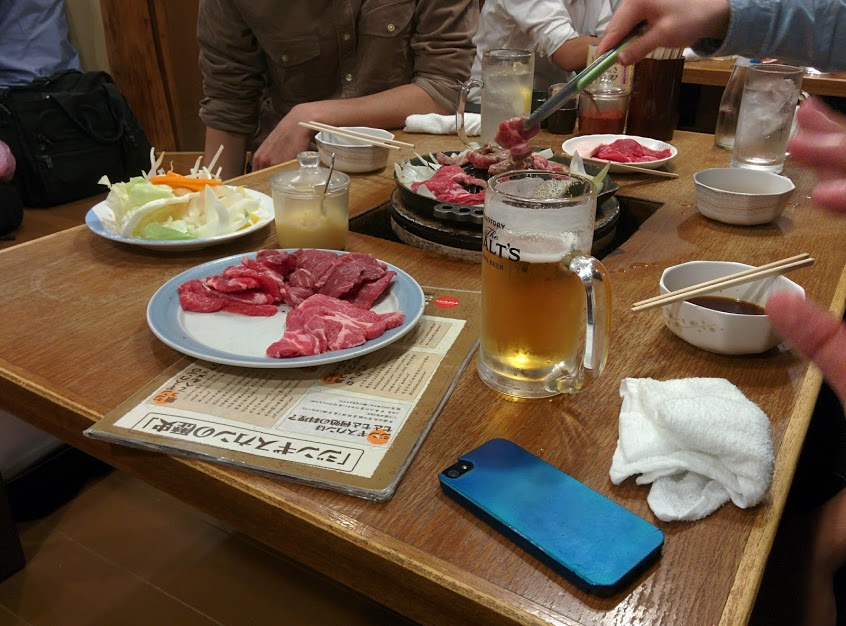
\includegraphics[width=0.45\linewidth]{welcome-party-2}
    }
    \subfigure[กระทะร้อนเจงกิสข่าน]{
        \label{Fig:welcome-party:3}
        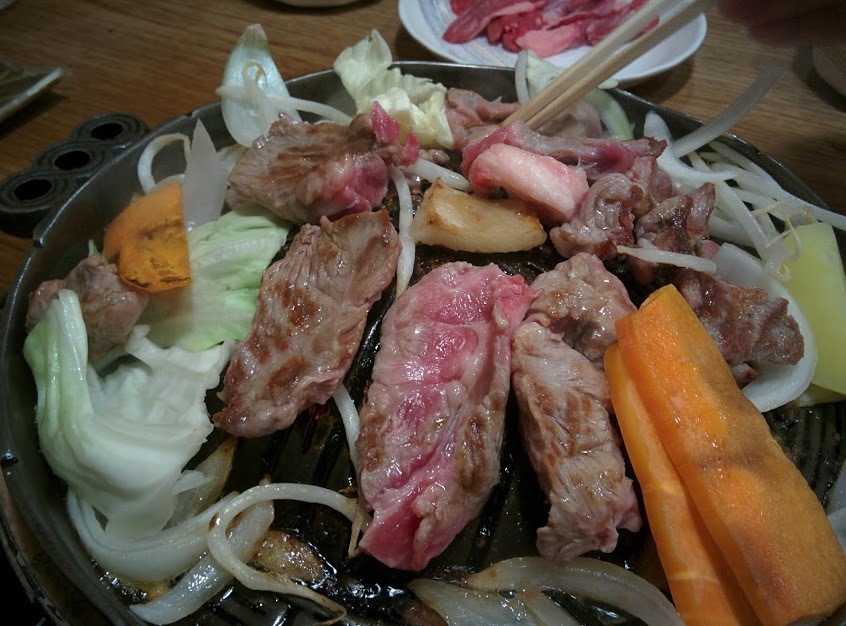
\includegraphics[width=0.45\linewidth]{welcome-party-3}
    }
    \caption{ภาพระหว่างงานเลี้ยงต้อนรับ}
    \label{Fig:welcome-party}
\end{figure}

นอกจากงานเลี้ยงต้อนรับแล้วยังมีงานเลี้ยงต้อนรับนักศึกษาปีสามที่เข้าเป็นสมาชิกใหม่ในห้องทดลองนี้อีกด้วย ซึ่งงานนี้จัดรวมเป็นงานเลี้ยงอำลาตัวผมพร้อม ๆ กันเนื่องจากจัดใกล้วันสิ้นสุดการฝึกงาน งานเลี้ยงจัดในห้องทดลองพร้อมด้วยอาหารหลากหลายชนิด งานไม่มีกิจกรรมอะไรมากมายเป็นเพียงการกินเลี้ยงเพื่อทำความรู้จักกับสมาชิกใหม่ของห้องทดลองและนั่งเล่นเกมด้วยกินตามที่แสดงในภาพ~\ref{Fig:farewell-party}

\begin{figure}[!h]
    \centering
    \subfigure[อาหารต่าง ๆ ในงานเลี้ยง]{
        \label{Fig:farewell:1}
        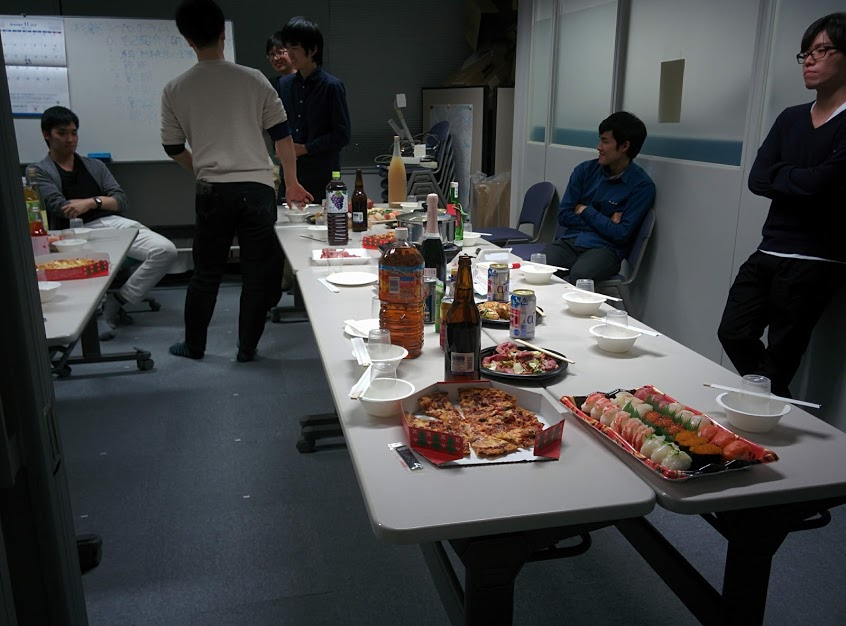
\includegraphics[width=0.8\linewidth]{farewell-party-1}
    }
    \subfigure[สมาชิกในห้องทดลองระหว่างเล่นเกมในงานเลี้ยง]{
        \label{Fig:farewell:2}
        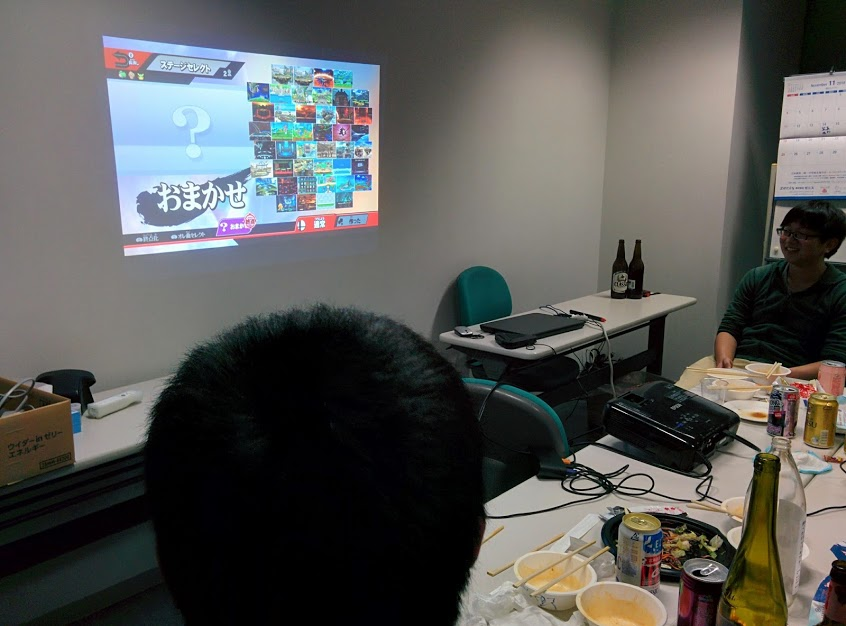
\includegraphics[width=0.8\linewidth]{farewell-party-2}
    }
    \caption{งานเลี้ยงอำลาและต้อนรับนักศึกษาปีสาม}
    \label{Fig:farewell-party}
\end{figure}

อธิบายเพิ่มเติมสำหรับงานเลี้ยงต้อนรับนักศึกษาปีสาม สำหรับห้องทดลองของคณะวิศวกรรมศาสตร์ที่ได้มาอยู่นี้จะมีการเปิดห้องทดลองให้นักศึกษาในคณะชั้นปีสามได้เข้าเยี่ยมชมห้องทดลองที่ตนเองสนใจก่อนจะเลือกเข้ามาเป็นสมาชิกในห้องทดลองที่เกี่ยวข้องกับงานที่สนใจจะทำ โดยงานที่สนใจจะทำจะกลายเป็นชิ้นงานจบการศึกษาคล้ายกับในมหาวิทยาลัยของไทย โดยในช่วงเวลานี้ของปีแต่ละห้องทดลองก็จะมีการโฆษณาห้องทดลองของตัวเองและเปิดโอกาสให้เข้าเยี่ยมชมงานภายในห้องทดลองว่าทำวิจัยเรื่องอะไร อย่างเช่นภาพ~\ref{Fig:ads} ที่เป็นป้ายเชิญเข้าชมห้องทดลองด้านเสียงและมีการใช้ตัวละครจากการ์ตูนเรื่อง Kemono Friend ประกอบให้น่าสนใจและดึงดูดมากขึ้น

\begin{figure}
    \centering
    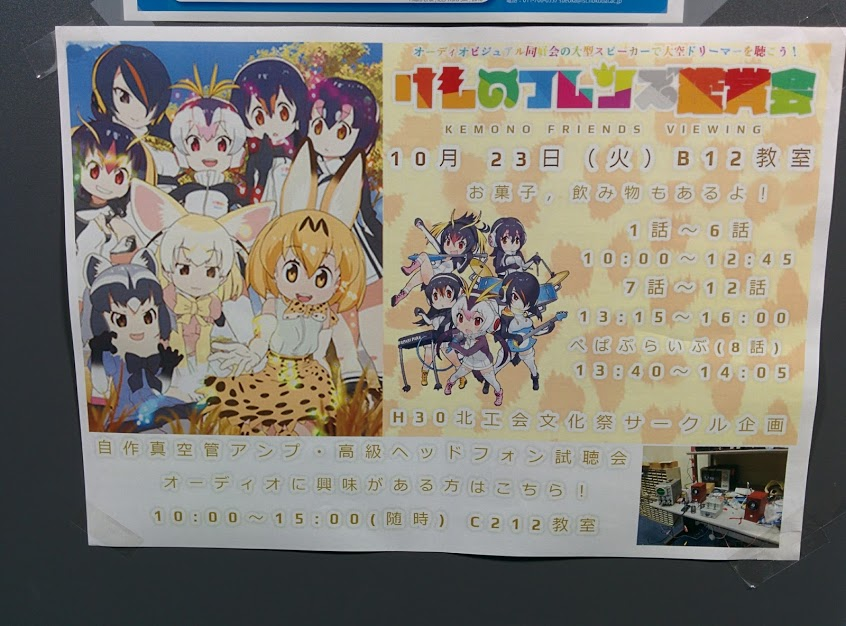
\includegraphics[width=0.8\linewidth]{ads}
    \caption{ป้ายเชิญชวนชมห้องทดลองโดยมีการใช้ตัวละครจากการ์ตูนประกอบให้น่าสนใจมากขึ้น}
    \label{Fig:ads}
\end{figure}

\clearpage 
\thispagestyle{empty}
\begin{center}
	\vspace*{\stretch{1}}
	\LARGE{\textbf{ภาคผนวก ค}}
	\vspace*{\stretch{1}}
\end{center}

\clearpage 
\thispagestyle{empty}
\begin{center}
    \vspace*{\stretch{1}}
    \LARGE{\textbf{ผลงานวิจัยที่ได้รับการตีพิมพ์}}
    \vspace*{\stretch{1}}
\end{center}

\addcontentsline{toc}{chapter}{ภาคผนวก\hspace{1ex}ค\hspace{2mm}ผลงานวิจัยที่ได้รับการตีพิมพ์}
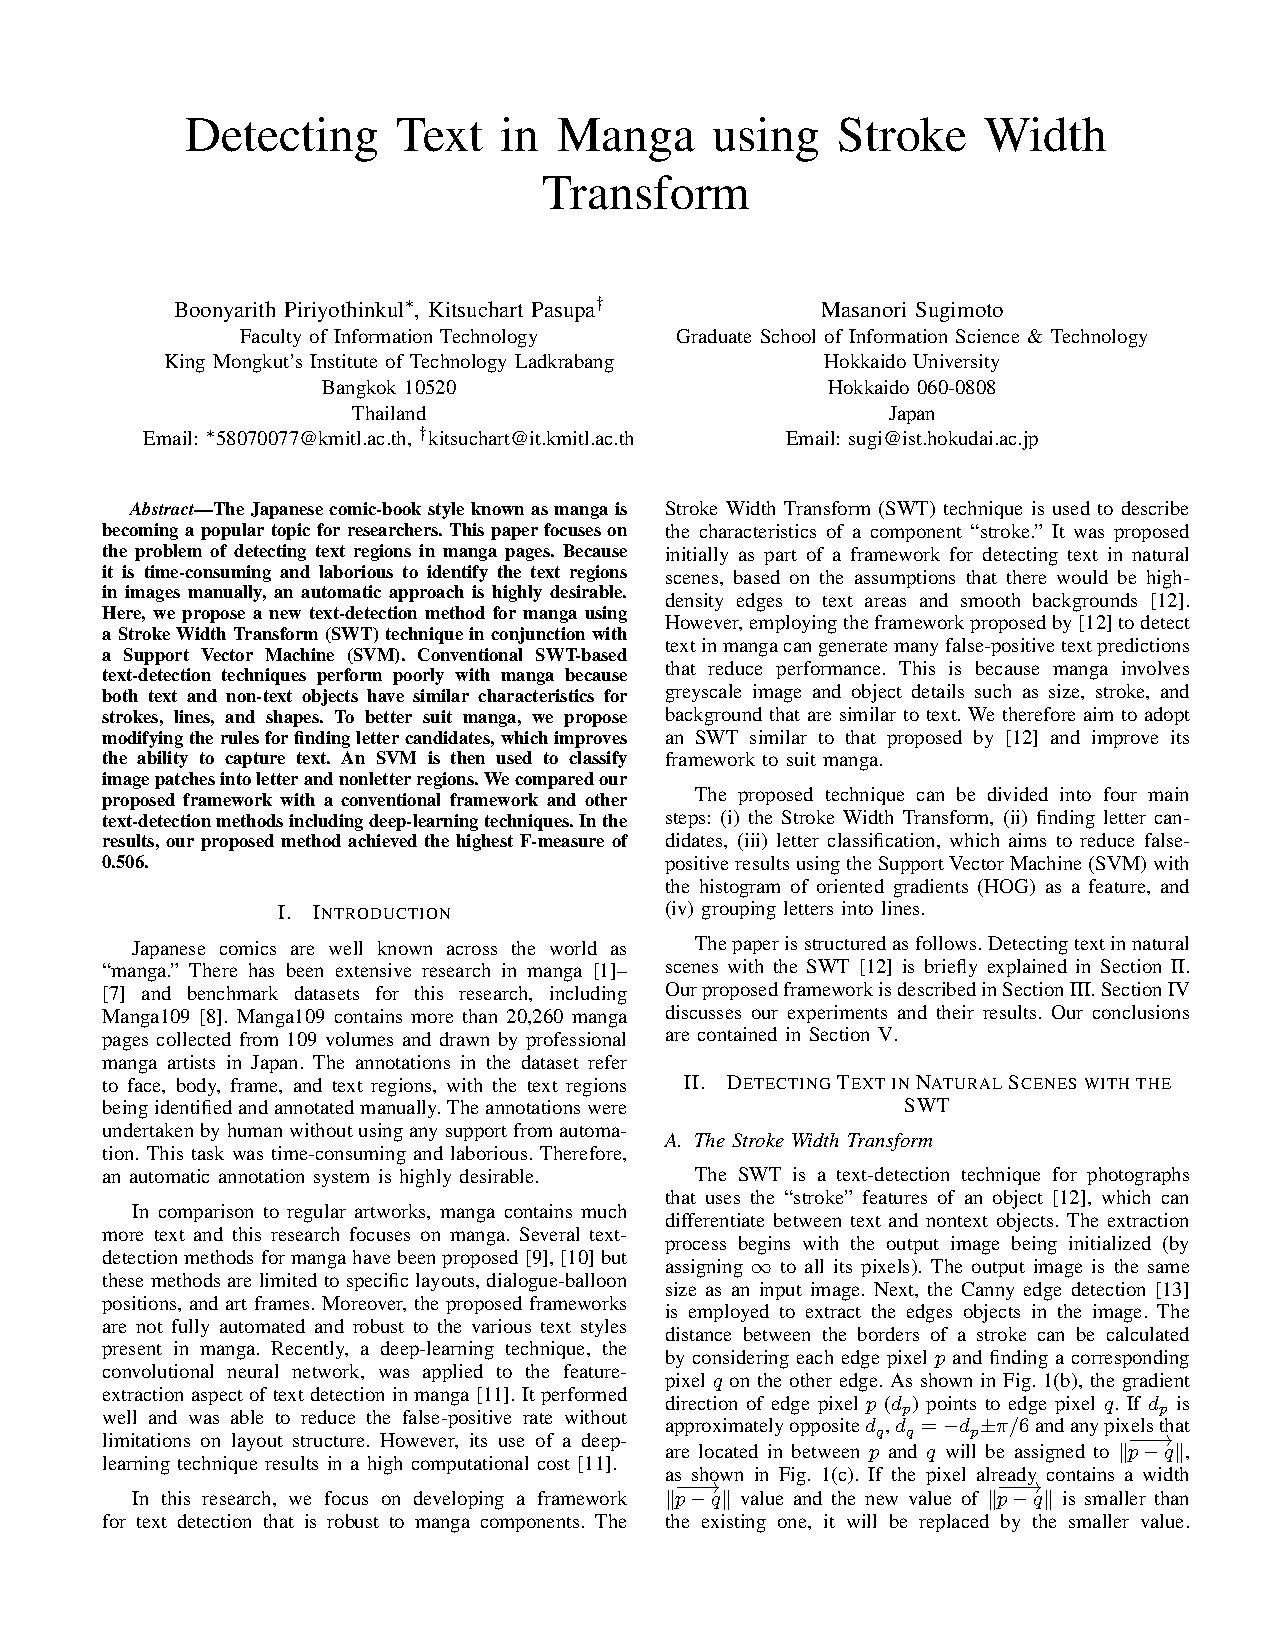
\includepdf[pages=-,pagecommand={}]{paper.pdf}